\subsection{Grunden}

\begin{frame}{Problemformulering, grunden}
\begin{equation*}
k\mathbf{n}\cdot\nabla T(\mathbf{r},t) = 
\begin{cases}
0&\mbox{, för rand mot berg} \\
h[T_\infty(t)-T(t)]&\mbox{, för rand mot luft} \\
U[T_{inne} - T(t)]&\mbox{, för rand mot grund}
\end{cases}
\end{equation*}

\uncover<2>{
\begin{figure}[hbp!]
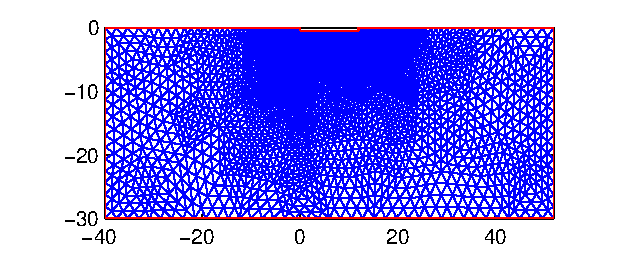
\includegraphics[height=0.4\textheight]{images/trifoundation.eps}
\end{figure}
}

\end{frame}

\begin{frame}{Energiflöden, grunden\\Hela året}

\begin{figure}[hpbt]
\centering
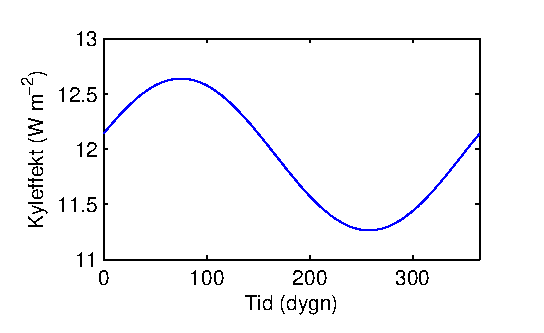
\includegraphics[height=5cm]{images/foundation.eps}
\caption*{Energiflödet genom grunden}
\end{figure}

\end{frame}
